\chapter{評価}
\label{chap:evaluation}

計測用のプログラムとして、与えられた整数$n$に対して$n$番目のフィボナッチ数を返す関数$fib(n)$を
C言語で実装した。

\begin{itembox}[l]{フィボナッチ関数のC言語による実装}
  \begin{verbatim}
    int fib(int n) {
      if (n <= 1) return 1;
      return fib(n - 1) + fib(n - 2);
    }
  \end{verbatim}
\end{itembox}

この関数をLLVM (Clang) 7.0でコンパイルして得られたWebAssemblyバイナリを、
\ref{chap:implementation}で述べたホストプログラムを通じてlibwasmにより
パースおよびアロケーションを行い、対応する関数を呼び出した。
また、同じ関数をホストプログラムの一部としてコンパイルし、直接呼び出した。

結果として、ESP32上でWebAssemblyバイナリを実行し、演算を行うことができた。
また、それぞれの場合において、\verb|fib|関数に与える引数\verb|n|を0から13まで
変化させ、各\verb|n|ごとの実行速度およびメモリフットプリントを計測し比較した。

\section{実行速度}

実行速度は、ESP-IDFが提供する\verb|esp_timer_get_time|関数を用いて計測した。
ESP-IDFにより実装されたプログラムは、起動後\verb|esp_timer_init|関数を自動的に呼び出し、
タイマーを初期化する。
\verb|esp_timer_get_time|関数は、タイマーを初期化してからの経過時間をマイクロ秒単位で返す。
フィボナッチ関数実行直前および実行直後に\verb|esp_timer_get_time|関数を呼び出し、差分を実行時間とした。

ネイティブ実行に対するWebAssemblyバイナリの実行時間について、引数\verb|n|を0から13まで変化させた際の推移を\ref{fig:exec_time}に示す。
横軸はフィボナッチ関数の引数$n$、縦軸は実行時間(マイクロ秒)を対数軸で示した片対数グラフである。

本実装およびネイティブ実行の双方において、$n=0$および$n=1$の時は定数を返すのみのため、引数による実行時間の変化がない。
定数を返す処理においては、本実装の実行時間はネイティブ実行の約260倍だった。

また、本実装およびネイティブ実行の双方において、実行時間は指数的に上昇している。
$n>2$にの場合において、…。

\begin{figure}[htbp]
  \caption{実行速度の変化とその比較}
  \label{fig:exec_time}
  \begin{center}
    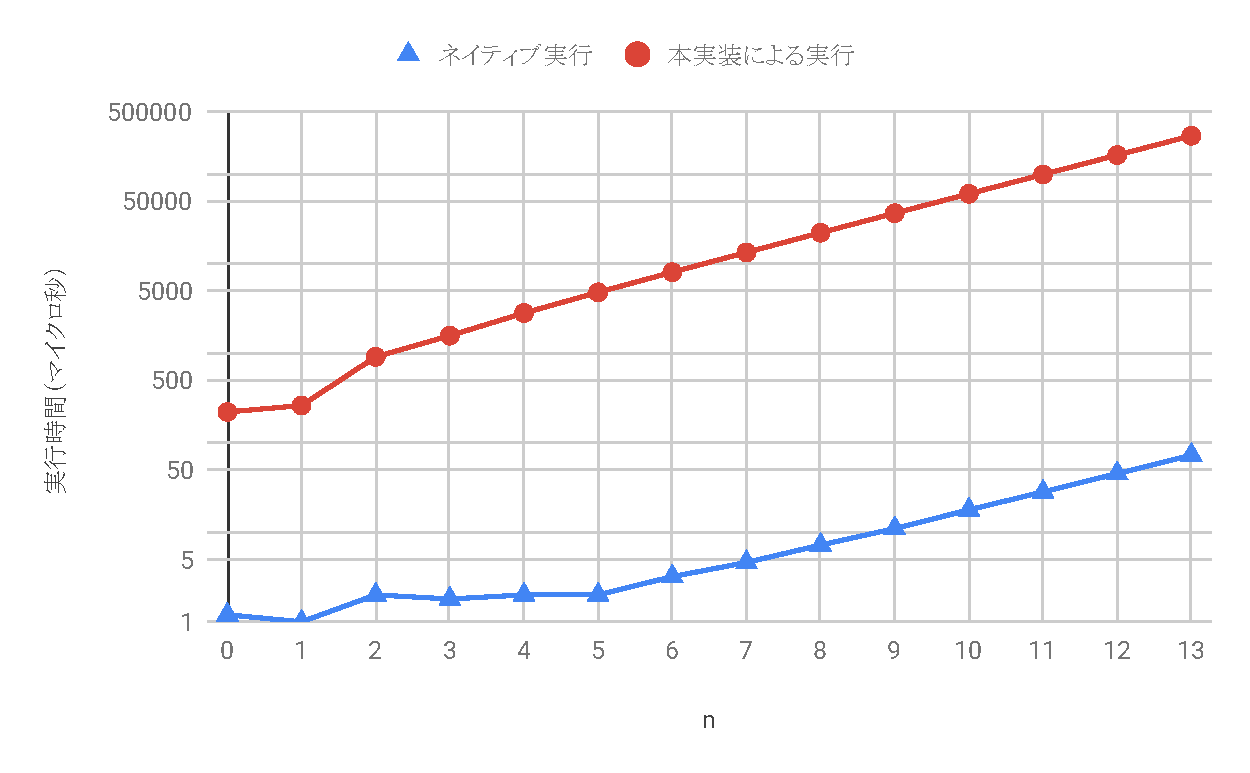
\includegraphics[bb=0 0 600 370,width=12cm]{img/fib_time.pdf}
  \end{center}
\end{figure}

\section{メモリフットプリント}

また、同プログラムについて、FreeRTOSが提供する\verb|xPortGetMinimumEverFreeHeapSize|
関数を用いてヒープ領域に確保されるメモリの最大量を計測した。

\verb|xPortGetMinimumEverFreeHeapSize|関数は、ブート以降未確保のヒープ領域が最小になった
時点でのサイズを返す。
ここで、モジュールのアロケーション後に\verb|xPortGetMinimumEverFreeHeapSize|関数で計測した値を0とし、
フィボナッチ関数を実行した後の同関数が返す値との差分を、関数実行のメモリフットプリントとした。

引数\verb|n|を0から13まで変化させた際の、関数実行のメモリフットプリントの推移を\ref{fig:heap_size}に示す。

\begin{figure}[htbp]
  \caption{メモリフットプリントの推移とその比較}
  \label{fig:heap_size}
  \begin{center}
    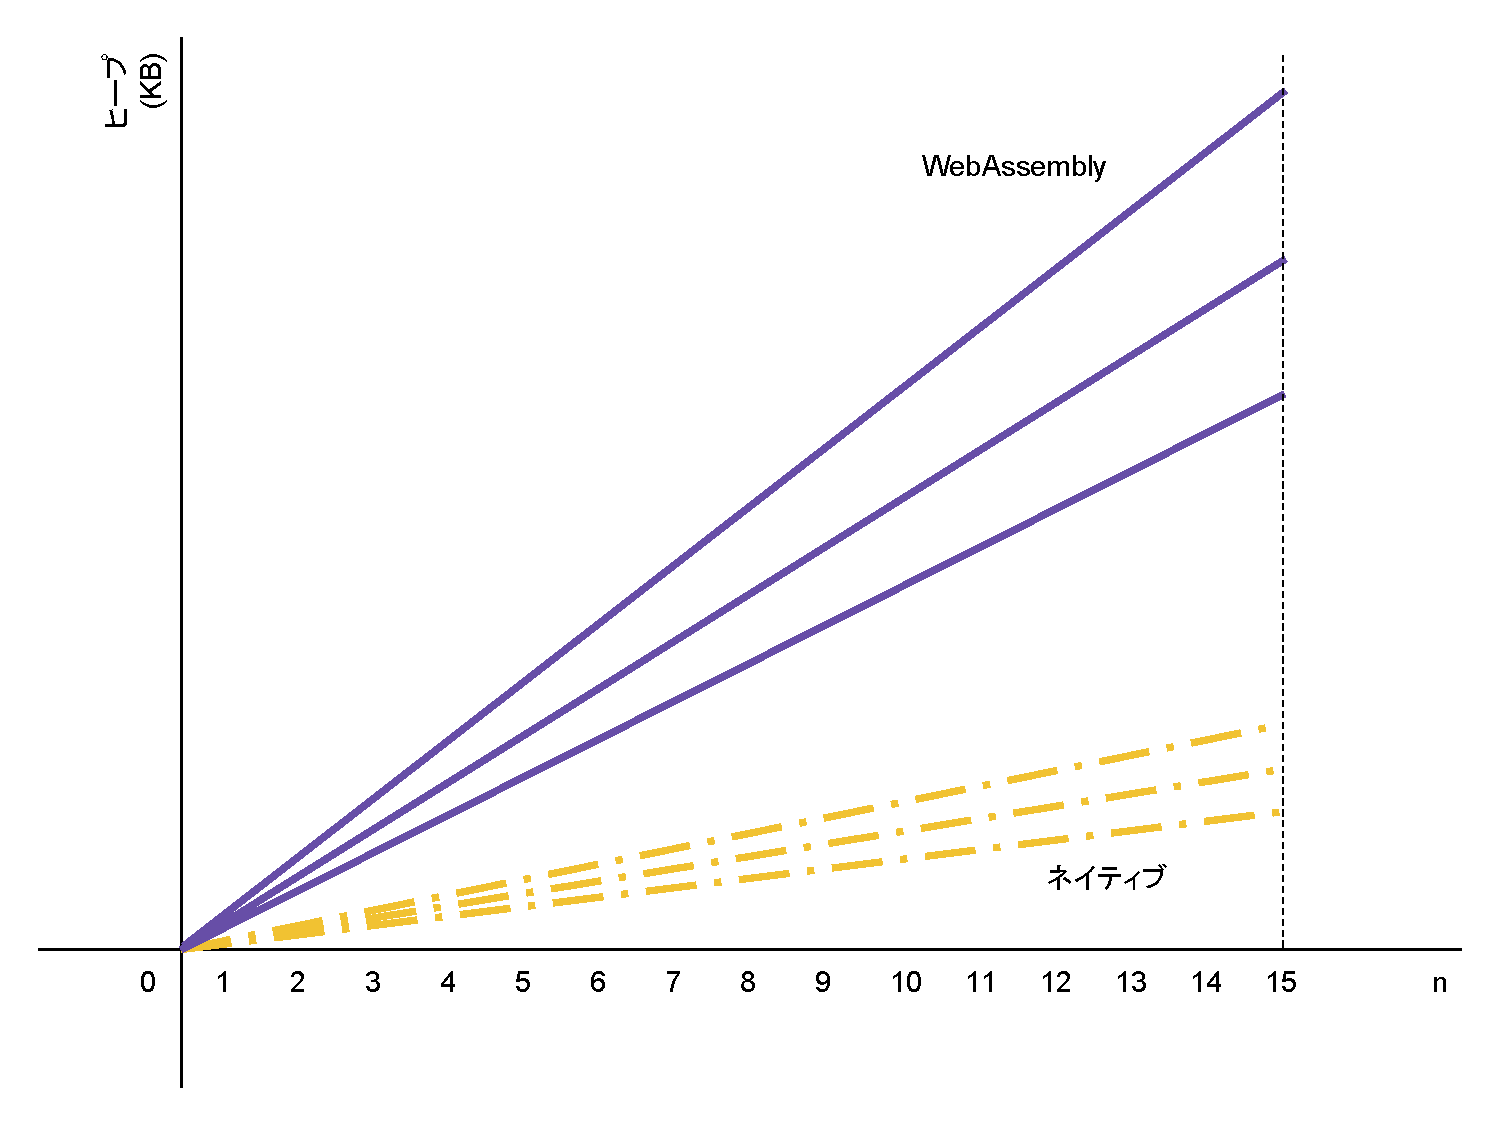
\includegraphics[bb=0 0 600 370,width=12cm]{img/heap_size.pdf}
  \end{center}
\end{figure}

実行速度と同じく、$n=0$および$n=1$の時は一定のメモリフットプリントだった。
$n=2$以降は208バイトずつ上昇していった。
